\documentclass[letterpaper, oneside, 11pt]{book}
\usepackage[left=1in, right=1in, top=0.75in]{geometry}
\usepackage[svgnames]{xcolor}
\usepackage{float}
\usepackage{graphicx}
\usepackage{setspace}
\usepackage{acronym}
\usepackage[sfdefault]{roboto}
\usepackage{xcolor}
\usepackage{sectsty}
\usepackage[colorlinks=true, linkcolor=gray]{hyperref}
\usepackage[utf8]{inputenc}
\usepackage{hyperref}
\usepackage{tabularx}
\usepackage{longtable}
\usepackage{glossaries}

\setacronymstyle{long-short-desc}
\loadglsentries{defn}
\makenoidxglossaries

\setcounter{secnumdepth}{3}
\definecolor{MyBlue}{rgb}{0.03, 0.27, 0.49}
\definecolor{bluekeywords}{rgb}{0.13,0.13,1}
\definecolor{greencomments}{rgb}{0,0.5,0}
\definecolor{turqusnumbers}{rgb}{0.17,0.57,0.69}
\definecolor{redstrings}{rgb}{0.5,0,0}
\definecolor{battleshipgrey}{rgb}{0.43, 0.5, 0.5}
\definecolor{graybkgrnd}{rgb}{0.5,0.5,0.5}
\chapterfont{\color{MyBlue}}
\sectionfont{\color{MyBlue}}
\subsectionfont{\color{MyBlue}}
\setlength{\parindent}{0pt}

\begin{document}
%%========================================================================
\begin{titlepage}
	\raggedleft
	\begin{figure}[H]
	\centering
		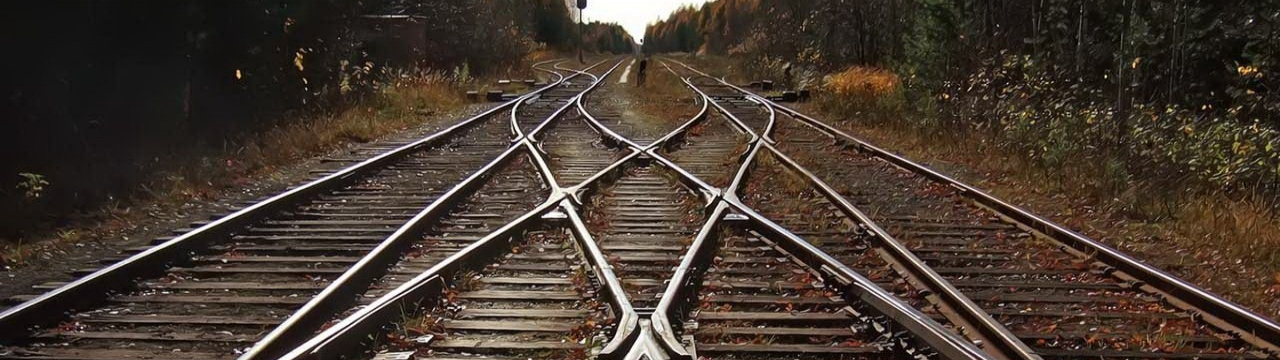
\includegraphics[scale=1.53]{railway_track.jpg}
	\label{fig:track}
\end{figure}
	\vspace*{0.167\textheight}
	\textbf{\LARGE Microcontrollers Design and Implementation}\\[\baselineskip]
    \textbf{\textcolor{MyBlue}{\Huge R\Large ailway \Huge A\Large dministration and \Huge I\Large nformation \Huge L\Large ogical \Huge S\Large ystem}}\\[\baselineskip]
	{\Large \textit{RAILS for Model Railroads}}
	\vfill
    \vspace*{\baselineskip}
	{\small David Bristow}

	{\small Version 1.0.1}
	
	{\small \today}
	\vspace*{3\baselineskip}
\end{titlepage}
%%========================================================================
\tableofcontents
%% copyright notice
\copyright David Bristow\\
%%========================================================================
\chapter{Microcontrollers for RAILS}
\section{Introduction}
\gls{rails} is a software model and implementation of an automated system to assist the model railroader achieve realism in the operation of a model railroad.
There are four user interface \gls{spa} that provide different aspects of rails they are:
\begin{itemize}
  \item \gls{rsrm} allows the user to match a rfid tag to a rollingstock's road name and number;
  \item \gls{mrim} allows the user to create, update and delete model railroad assets, such as rolling stock;
  \item \gls{mppm} allows the user to enter information about their projects and purchases; and
  \item \gls{mrlm} allows the user to enter information about their layout and control elements of it.
\end{itemize}
\section{RSRM Components}
The implementation of \gls{rsrm} consists of the following micro-services components:
\begin{itemize}
\item \gls{rfid} Controller is a micro-controller that processes \gls{rfid} tags obtained from a \gls{rfid} reader and then publishes \gls{iot} messages to the \gls{mqtt} Broker;
\item \gls{mqtt} Broker is responsible for receiving \gls{rfid} and micro info messages, filtering them, posting to designated topics and sending messages to clients subscribing to topics. The subscribers and publishers bridge the \gls{mqtt} elements with the GUI applications. The broker handles \gls{iot} messages;
\item \gls{isrs} subscribes to \gls{rfid} messages and pushes them via a web-socket to the rsm component;
\item \gls{isms} that subscribes to micro controller startup and heartbeat messages, updating the micros collection via \gls{rlds};
\item \gls{rlds} provides \gls{rest} access to model railroad layout collections including micros;
\item \gls{rids} provides \gls{rest} access to railroad inventory collections including rollingstock;
\item MongoDB a NoSQL database program that stores data records as documents which are gathered in collections. A database stores one or more collections of documents;
\item \gls{mr} Data is the document repository, used by MongoDB, to store complete collections of items such as rollingstock, industries (producers and consumers), track elements, turnouts, projects, purchases, etc. in support of \gls{rails}; and
\item \gls{rsrm} is the \gls{spa} that allows a user to match a \gls{rfid} tag to a rollingstock's road name and number.
\end{itemize}
Figure \ref{fig:rsms-ms-components} depicts the micro-services used to create the rolling stock \gls{rfid} management subsystem.

\begin{figure}[H]
	\centering
		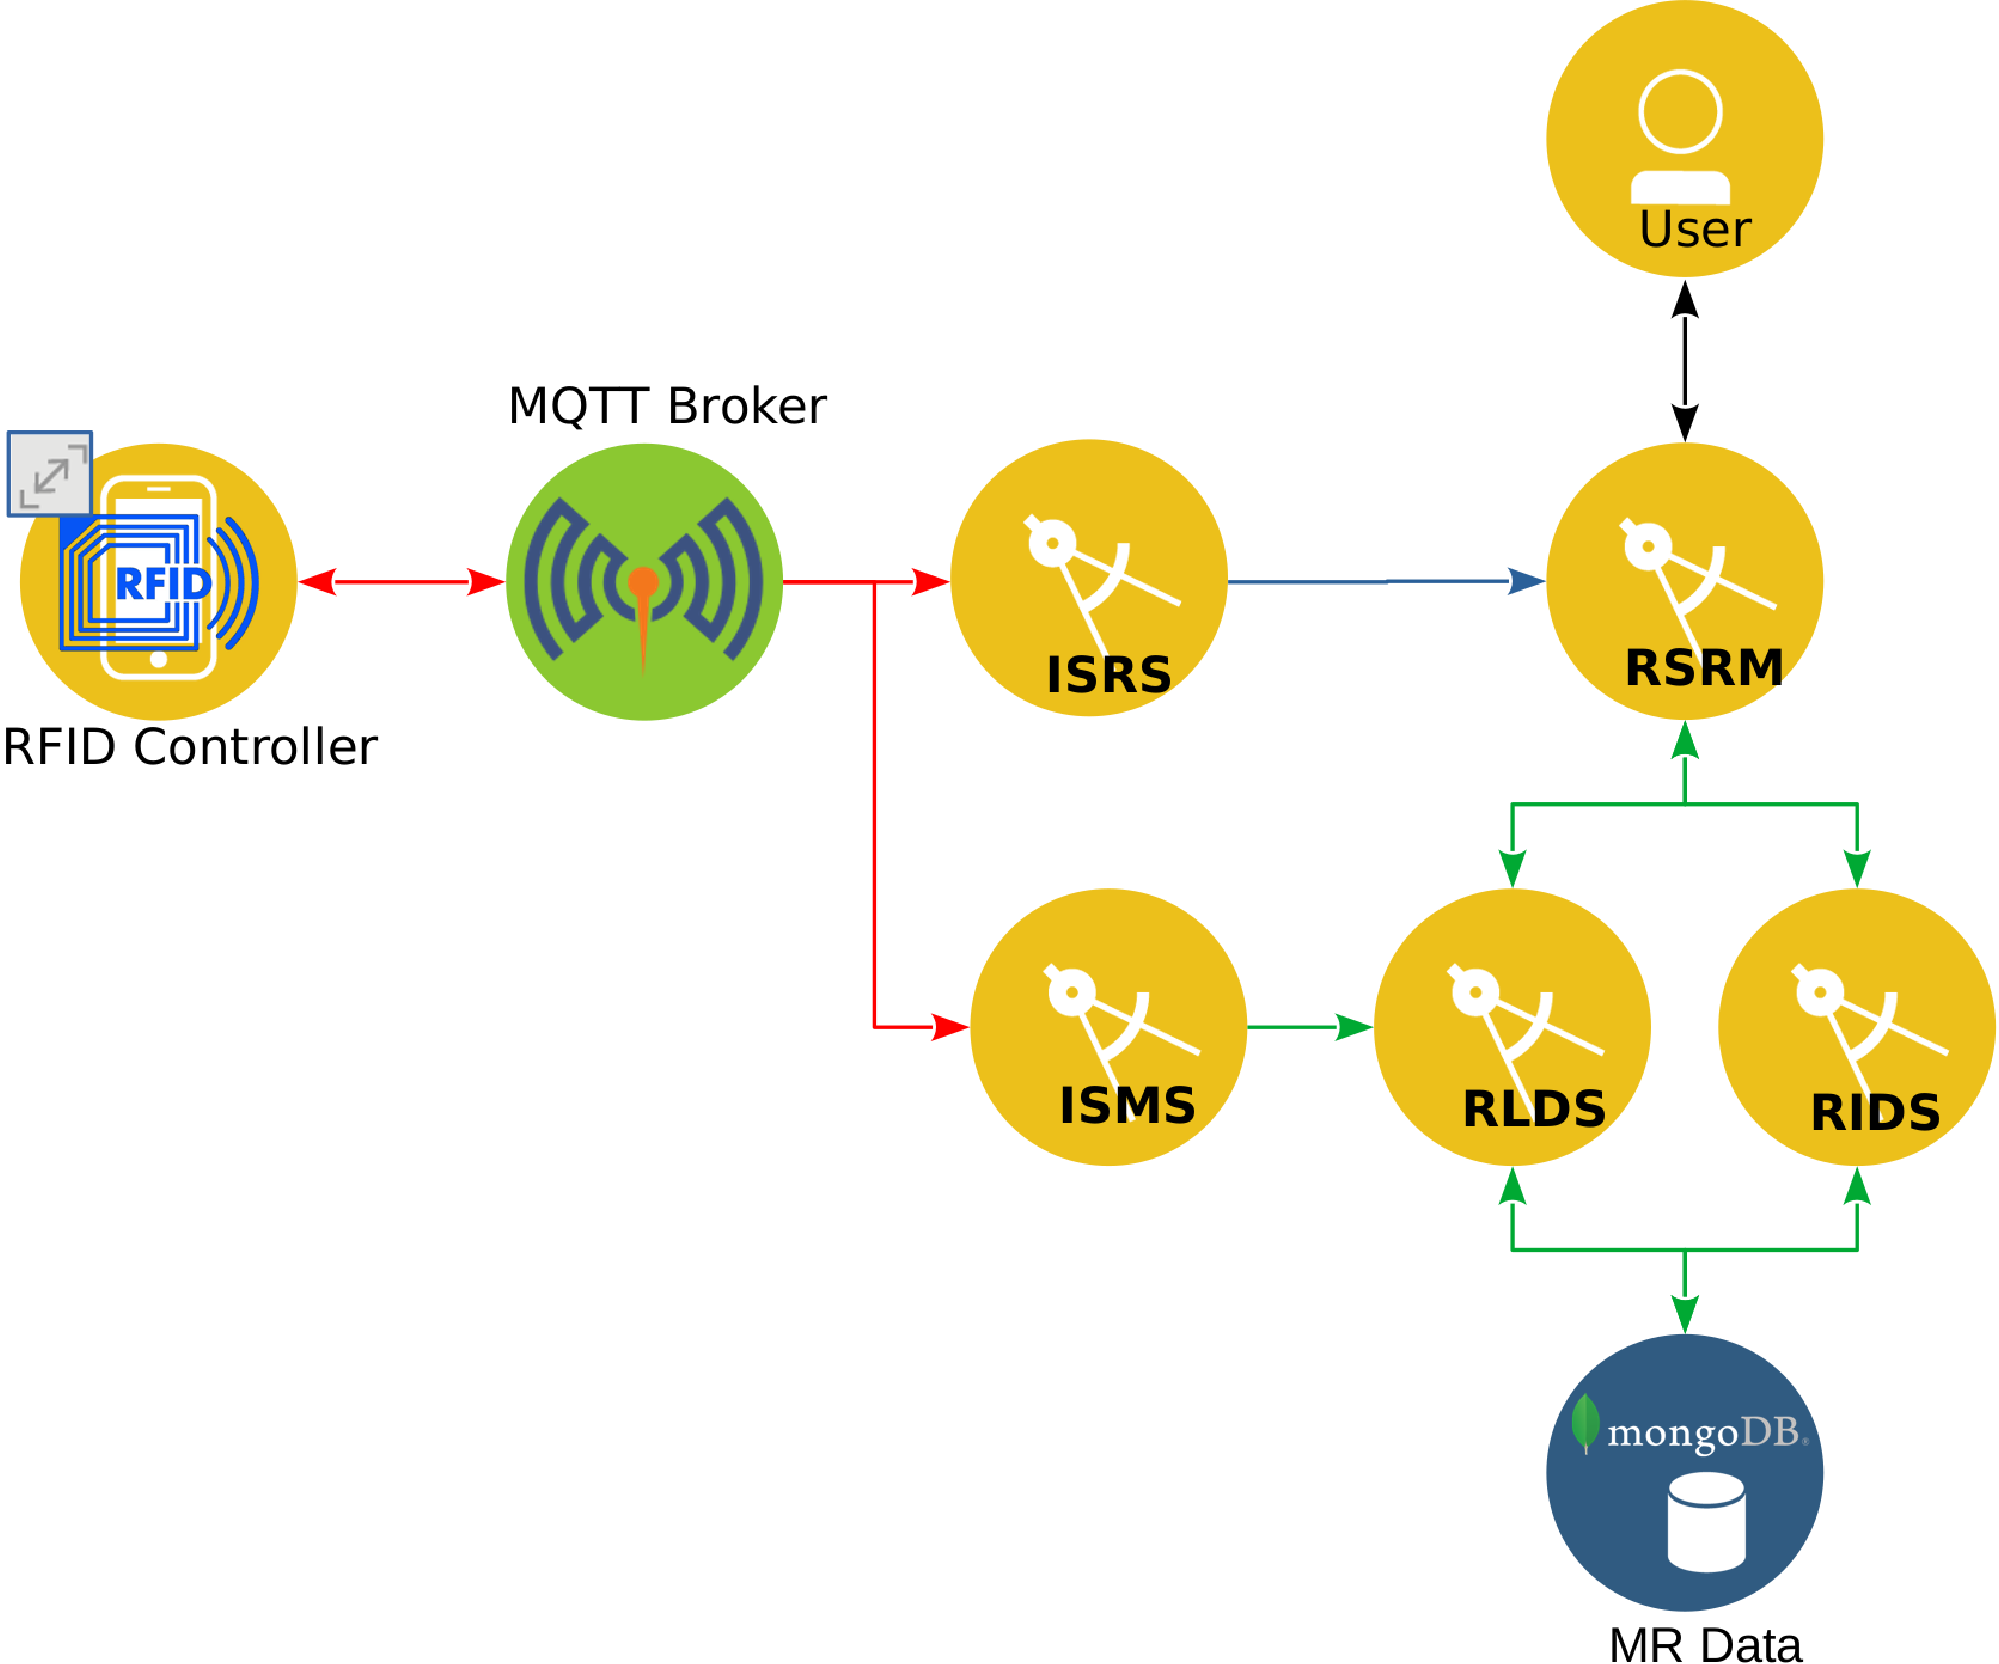
\includegraphics[scale=0.15]{../Images/rsms_microservices.png}
	\caption{Microservices Components}
	\label{fig:rsms-ms-components}
\end{figure}

Three system components that make up this subsystem:
\begin{itemize}
\item \gls{rfid} Controller is a micro-controller that processes \gls{rfid} tags obtained from a \gls{rfid} reader and then publishes \gls{iot} messages to the \gls{mqtt} Broker;
\item Network is a \gls{tcpip} communication medium that connects the \gls{rfid} Controller, \gls{mqtt} Broker and \gls{rsrm} components; and
\item Host is a computer that runs the \gls{mqtt} Broker and other \gls{rsrm} micro-services components.
\end{itemize}
Figure \ref{fig:rsms-system} depicts the systems components used to create the rolling stock \gls{rfid} management subsystem.

\begin{figure}[H]
	\centering
		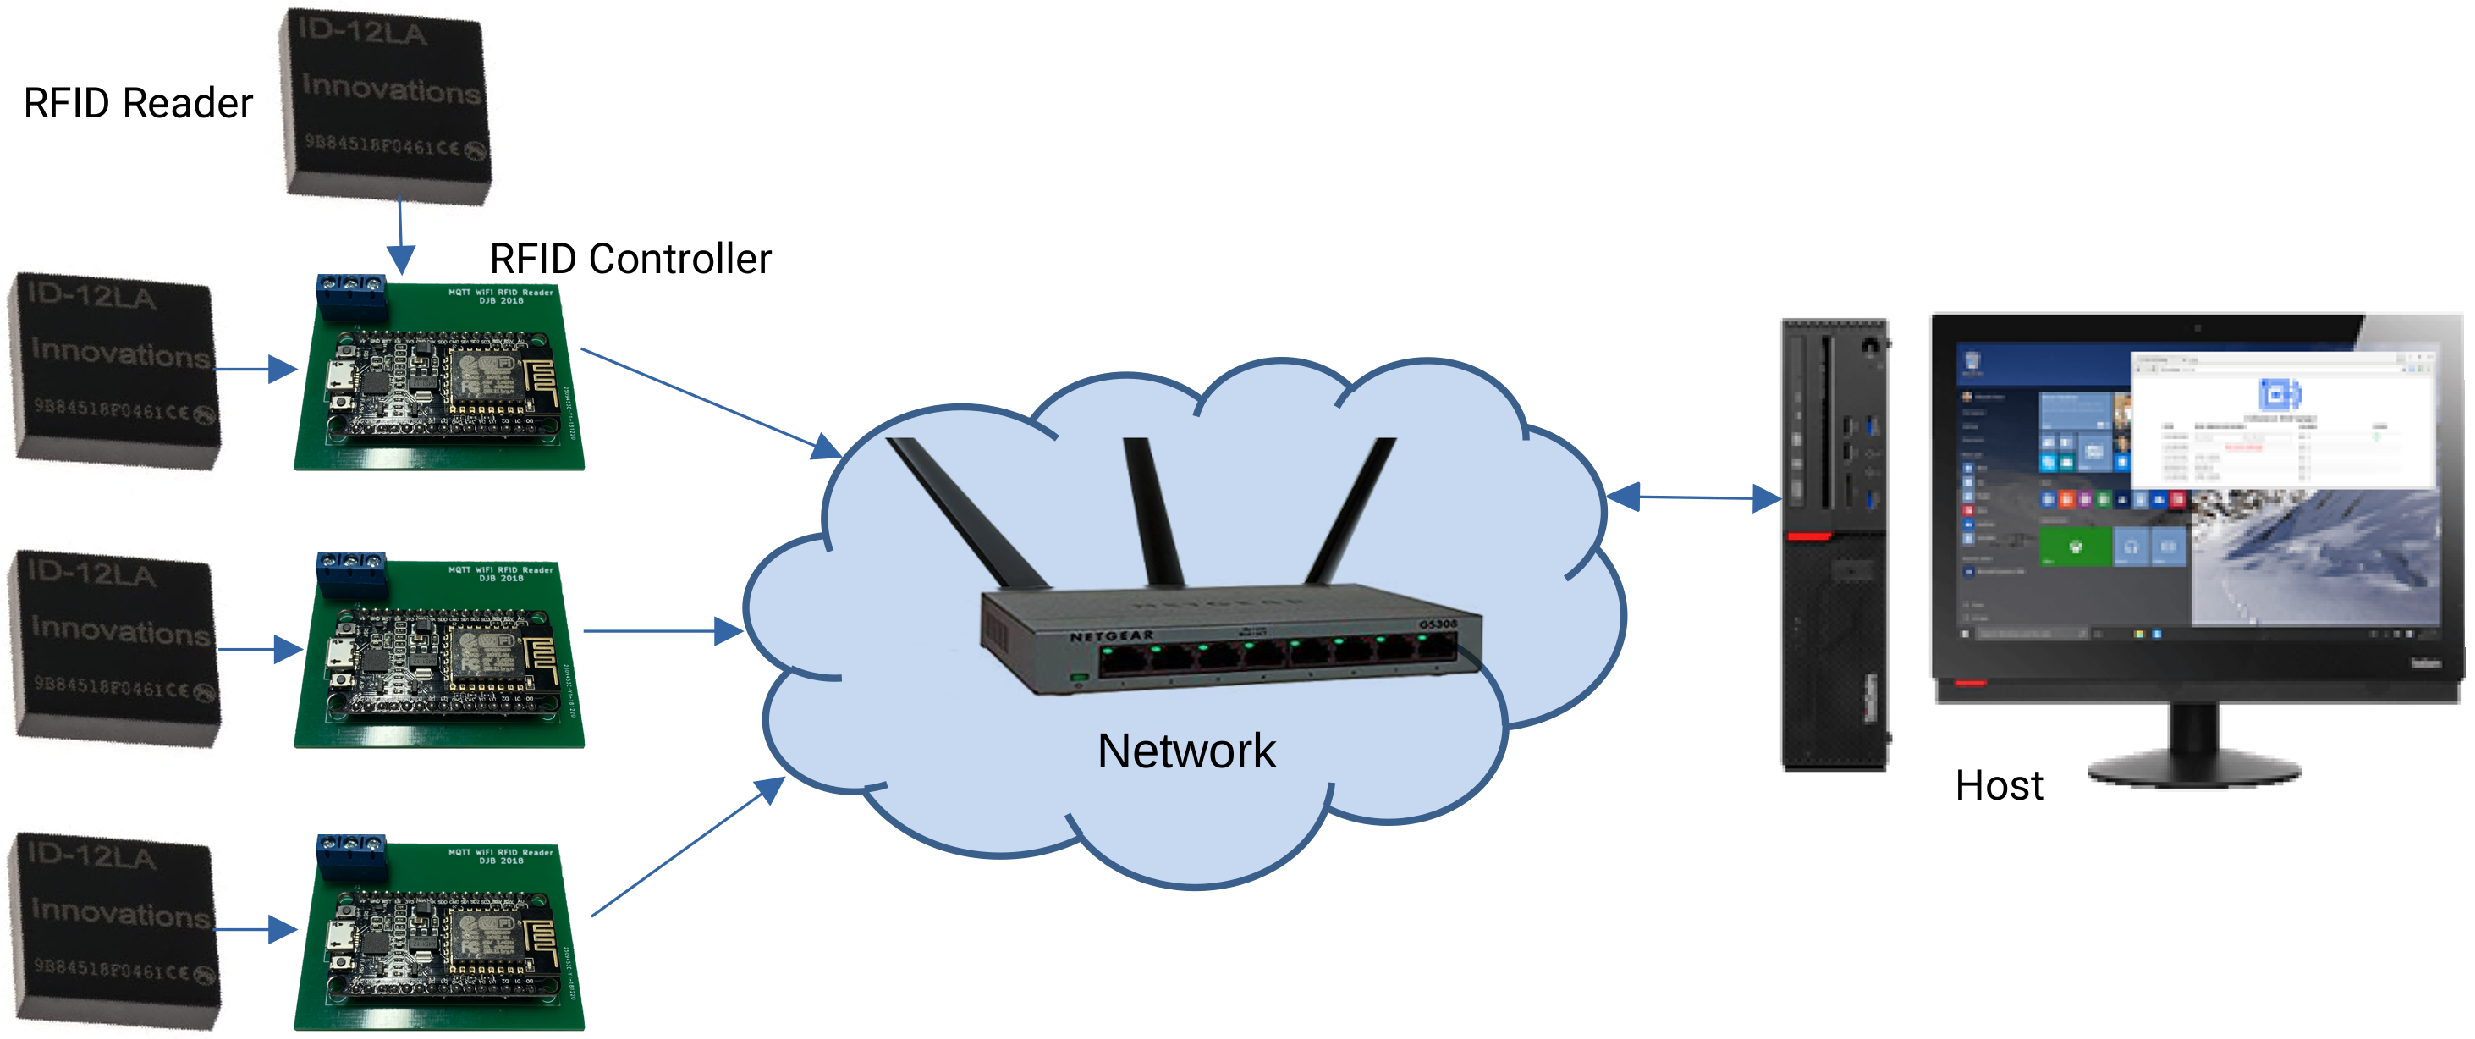
\includegraphics[scale=0.15]{../Images/rsms_system.png}
	\caption{RSMS System Components}
	\label{fig:rsms-system}
\end{figure}

\section{MRLM System Components}

Figure \ref{fig:mrlm-ms-components} depicts the micro-services used to create the \gls{mrlm} subsystem and figure \ref{fig:turnout-system} depicts it's logical architecture.

\begin{figure}[H]
	\centering
		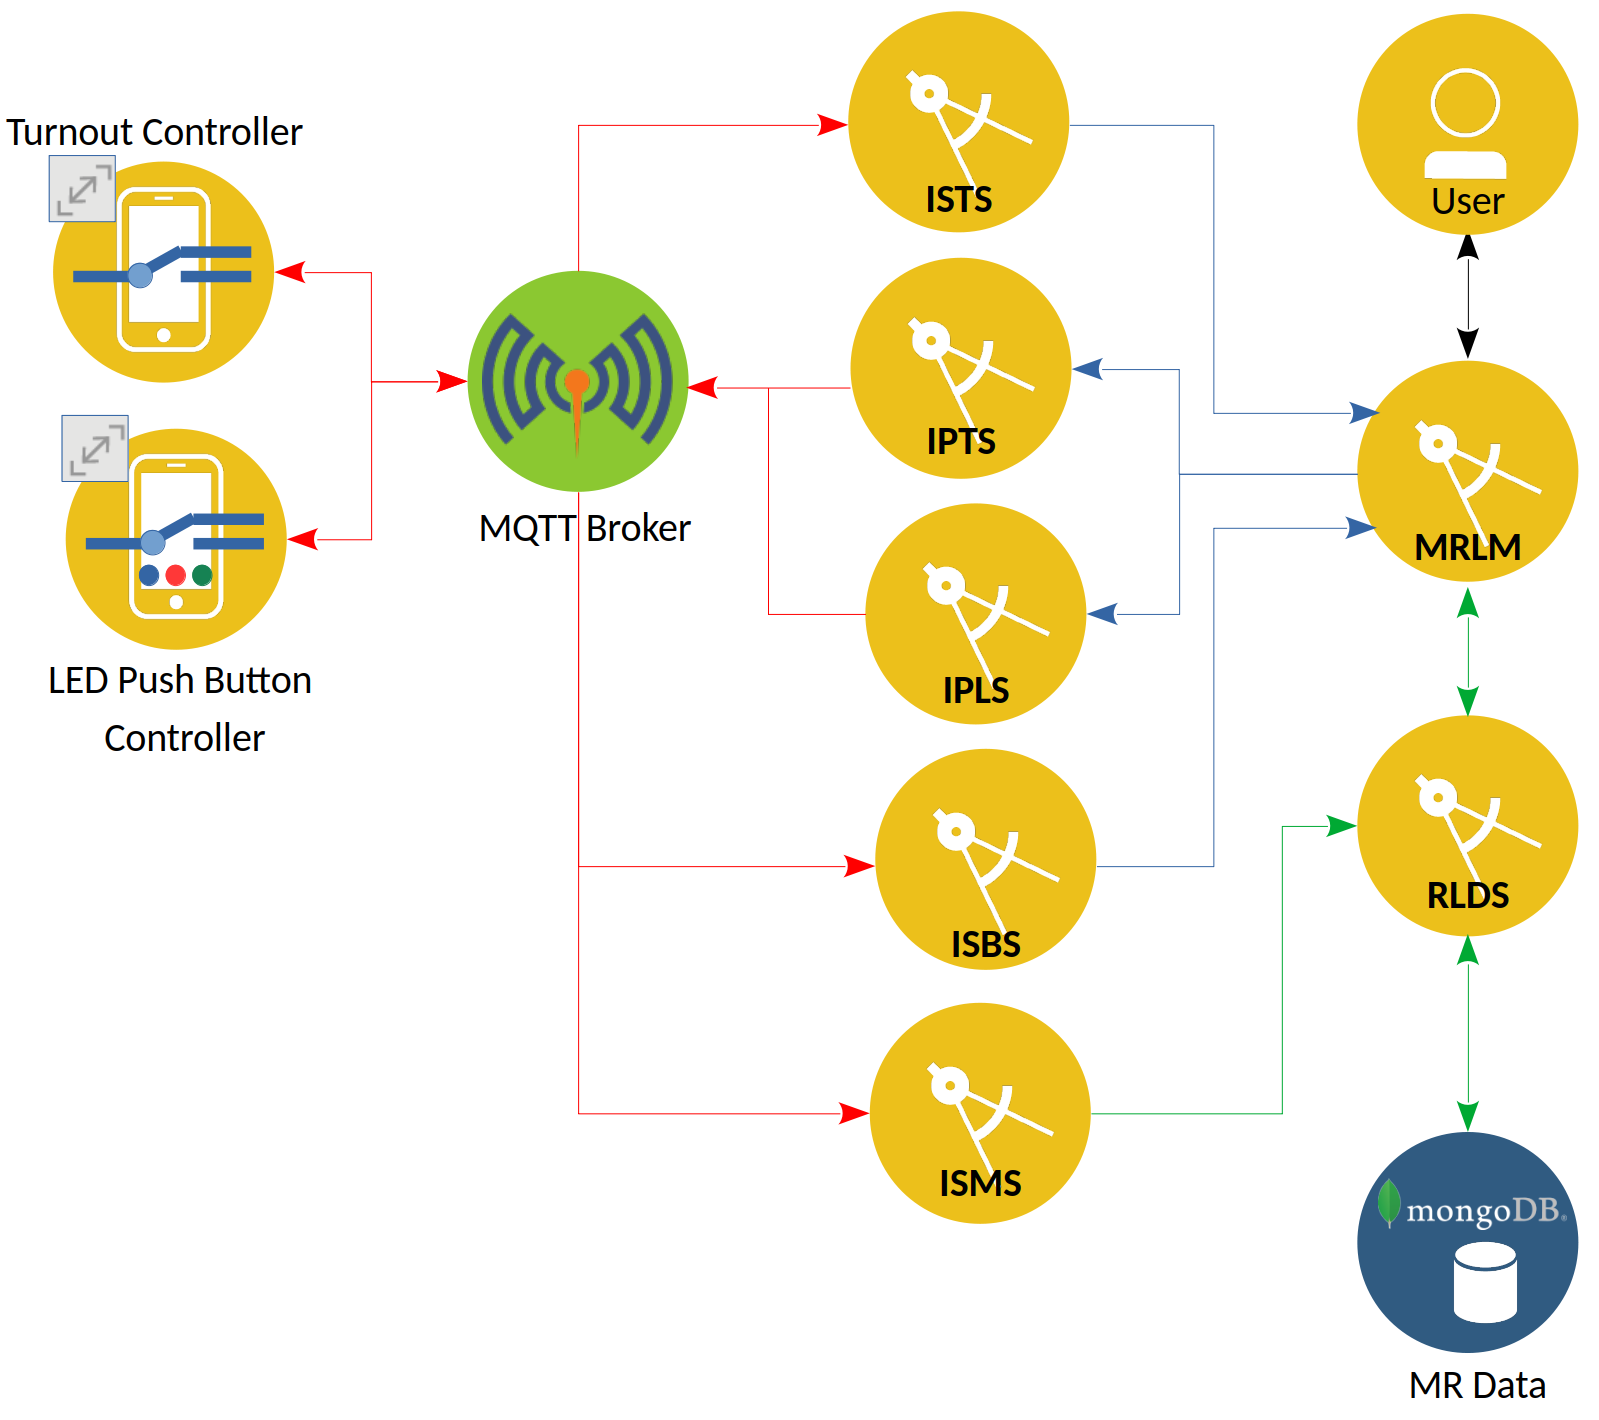
\includegraphics[scale=0.2]{../Images/mrlm_microservices.png}
	\caption{Microservices Components}
	\label{fig:mrlm-ms-components}
\end{figure}


\begin{figure}[H]
	\centering
		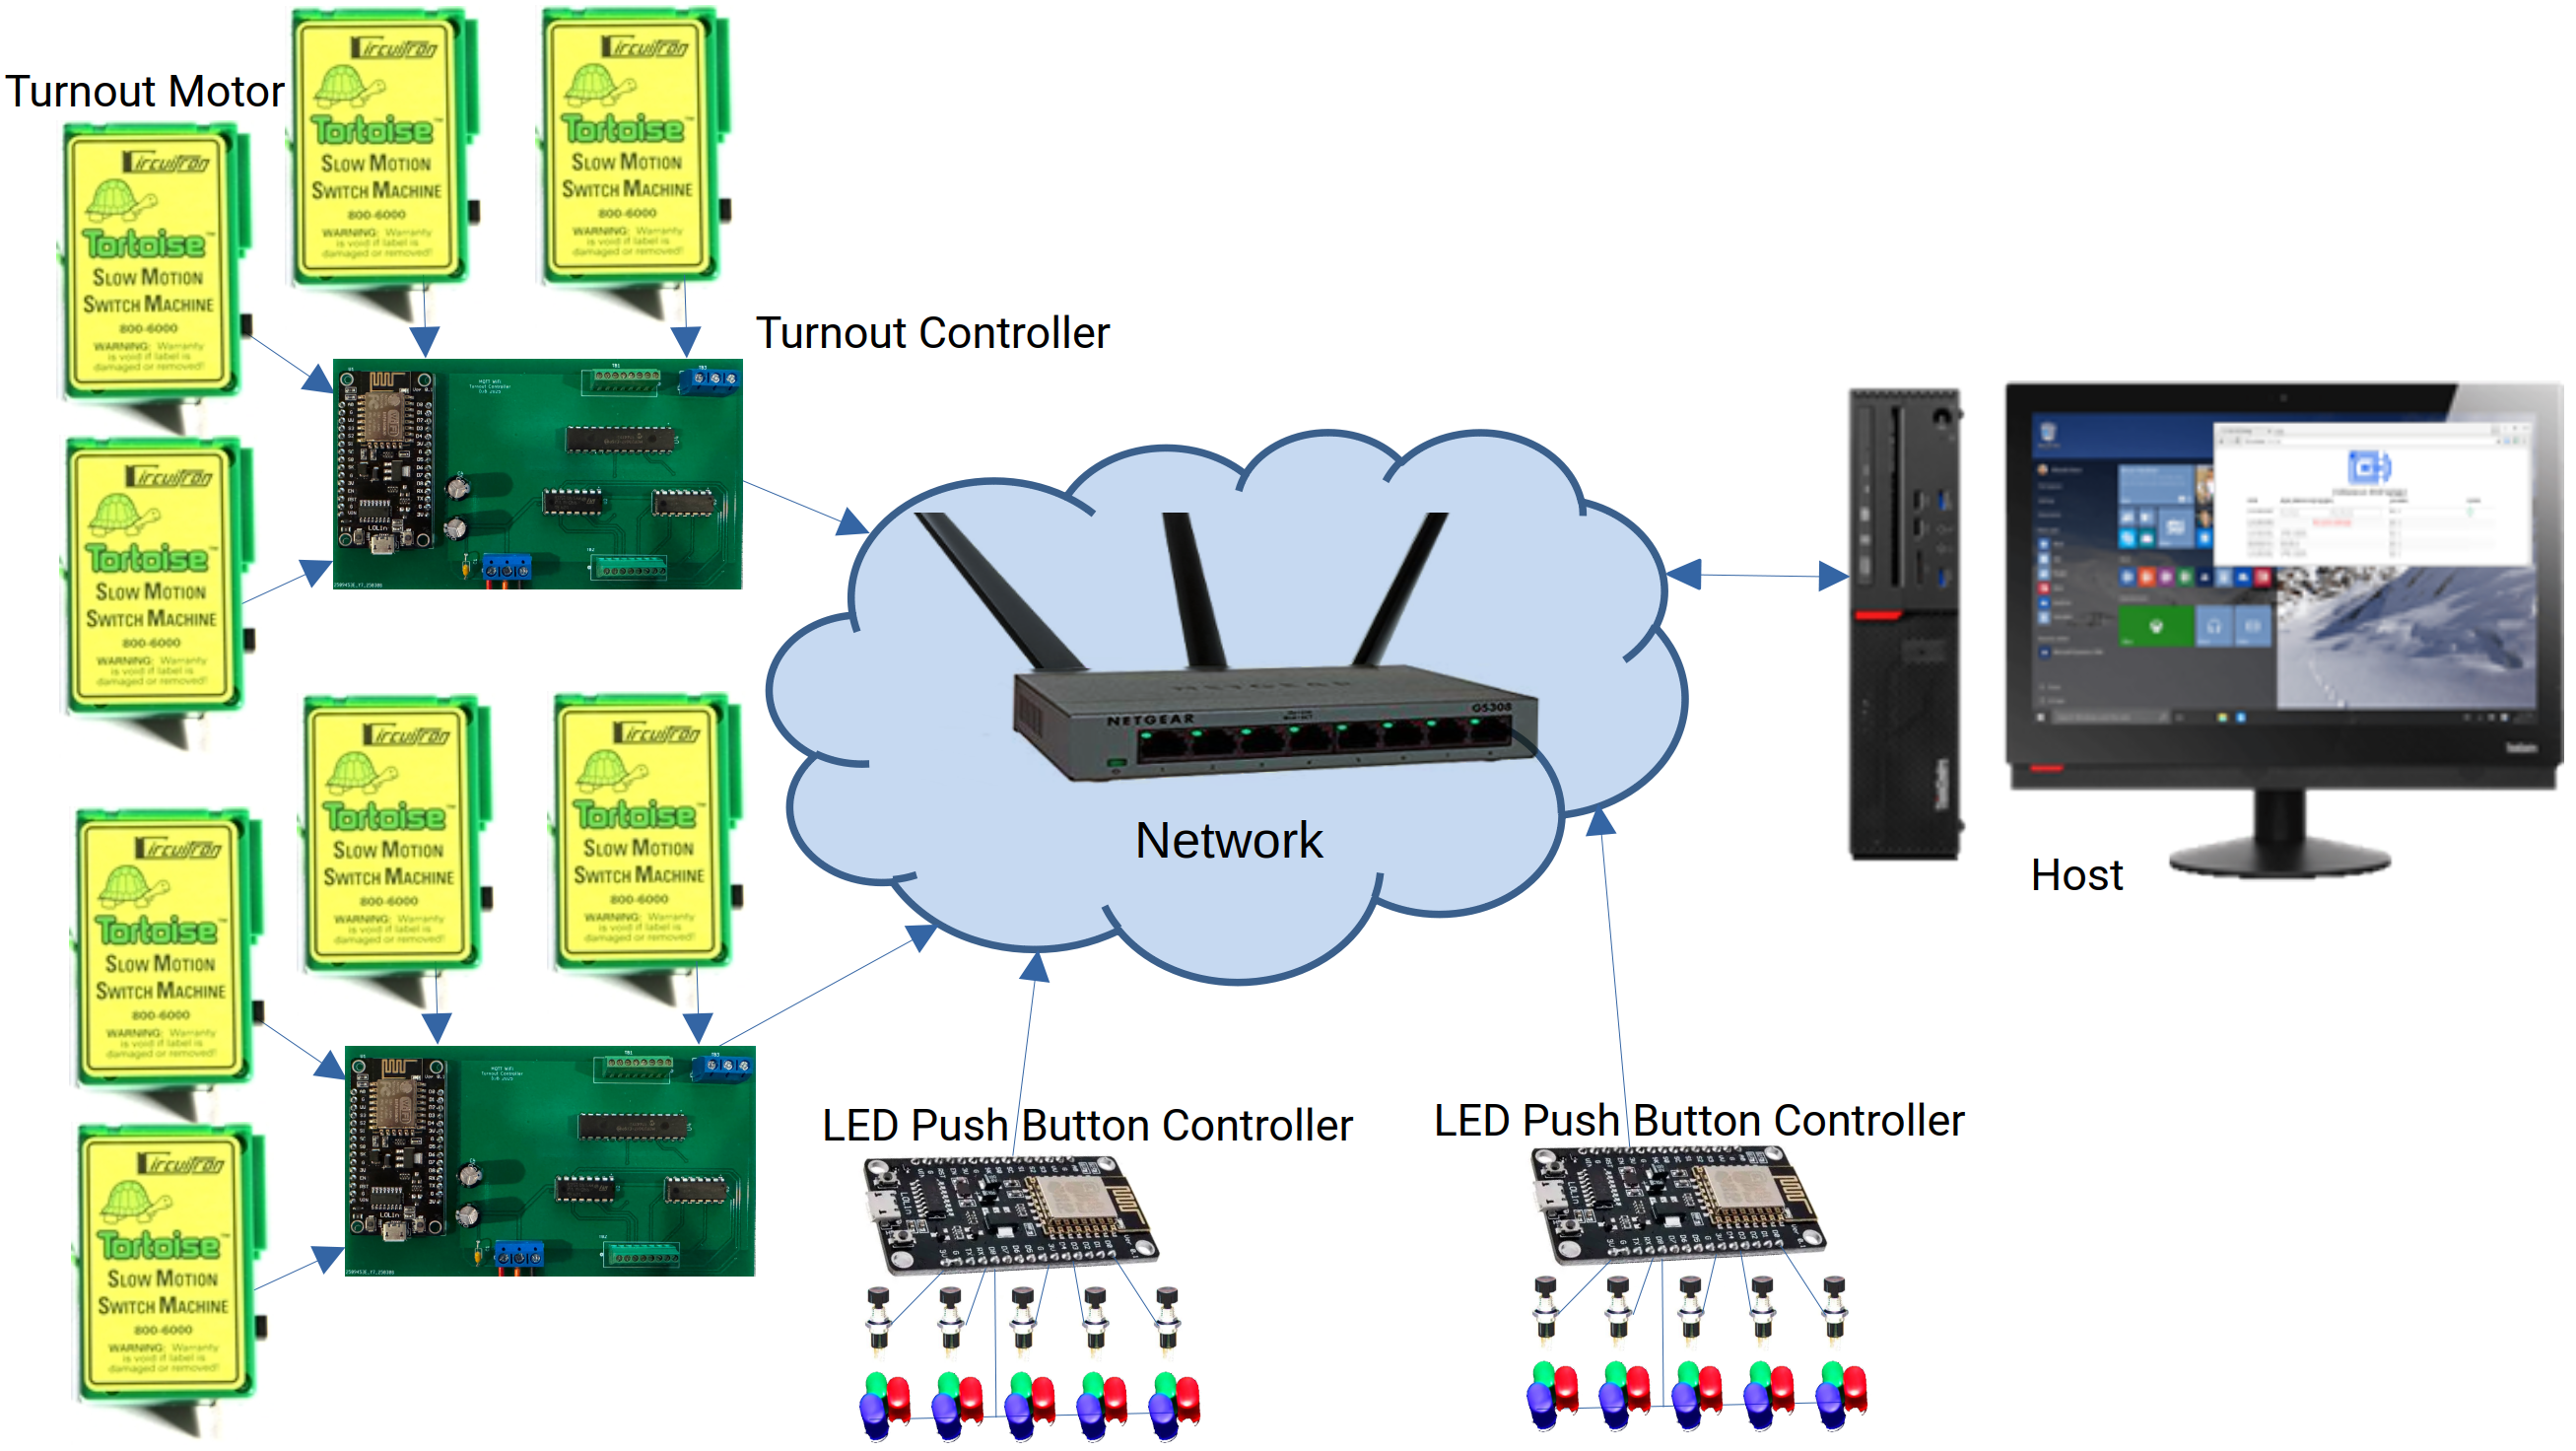
\includegraphics[scale=0.2]{../Images/mrlm_system.png}
	\caption{MRLM System Components}
	\label{fig:turnout-system}
\end{figure}

\chapter{RFID Microcontroller}
\section{Introduction}
The \gls{rfid} microcontroller is a versatile and compact system designed to interface with \gls{rfid} readers and process tag information efficiently. It acts as a bridge between \gls{rfid} 
hardware and software applications, enabling seamless communication and data exchange. Built around the NodeMCU, which is powered by the ESP8266 chip, the microcontroller 
offers robust processing capabilities and integrated \gls{wifi} connectivity. This makes it ideal for \gls{iot} applications where \gls{rfid} data needs to be transmitted over a network for further 
processing, monitoring, or storage. The system is designed to be reliable, scalable, and easy to integrate into various use cases, including access control, inventory management, asset tracking, 
and smart automation systems.
\section{Hardware}
\subsection{Schematic}
The schematic diagram in Figure \ref{fig:rfid-schematic} illustrates the design of the \gls{rfid} microcontroller circuit. It shows the connections between componentse and the terminal blocks for one or two \gls{rfid} readers. 
Each component is carefully integrated to ensure reliable recieving the tag information from the \gls{rfid} readers.

\begin{figure}[H]
  \centering
    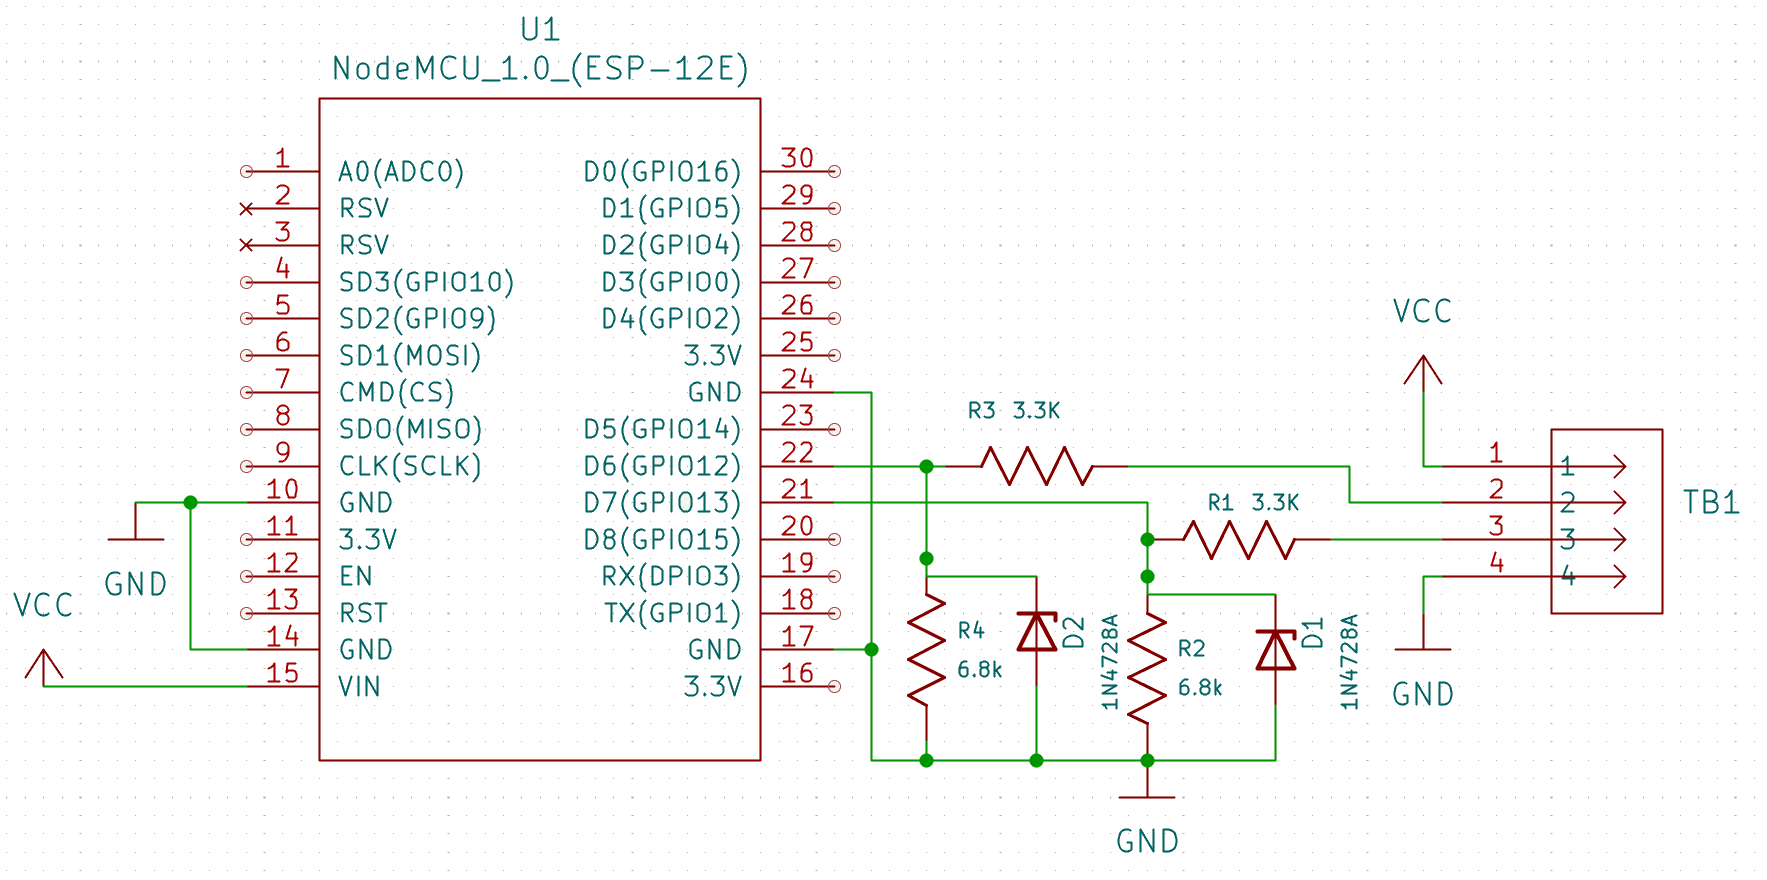
\includegraphics[scale=0.2]{../Images/rfid_schematic.png}
  \caption{RFID Microcontroller Schematic}
  \label{fig:rfid-schematic}
\end{figure}

The hardware used in the \gls{rfid} microcontroller circuit consists of several components that work together to enable the \gls{rfid} readers. The main components are:
\begin{itemize}
\item NodeMCU (U1) is the central microcontroller, an ESP8266, which will manage communication with the \gls{rfid} readers.
\item Resistors (R1, R2, R3, R4) are resistors crucial for voltage level shifting.
\item Zener Diodes (D1, D2) are diodes, along with the resistors, form a level shifting circuit.
\item TB1 Connector is the 4-pin connector where the \gls{rfid} readers are attached.
\end{itemize}
The NodeMCU (U1) is programmed to handle the communication with the \gls{rfid} readers through the \gls{i2c} protocol. The resistors (R1, R2, R3, and R4) are used in a level shifting circuit to ensure that the voltage levels between the 
NodeMCU and the \gls{rfid} readers are compatible. The diodes (D1 and D2) are used to protect against voltage spikes and ensure proper operation of the level shifting circuit. The TB1 connector is where the \gls{rfid} readers are connected to the microcontroller.

\subsection{PCB Design}
The \gls{pcb} design for the \gls{rfid} microcontroller is shown in Figure \ref{fig:rfid_pcb}. The PCB layout is designed to accommodate all the components mentioned in the schematic, ensuring proper 
connections and efficient routing of signals.

\begin{figure}[H]
  \centering
    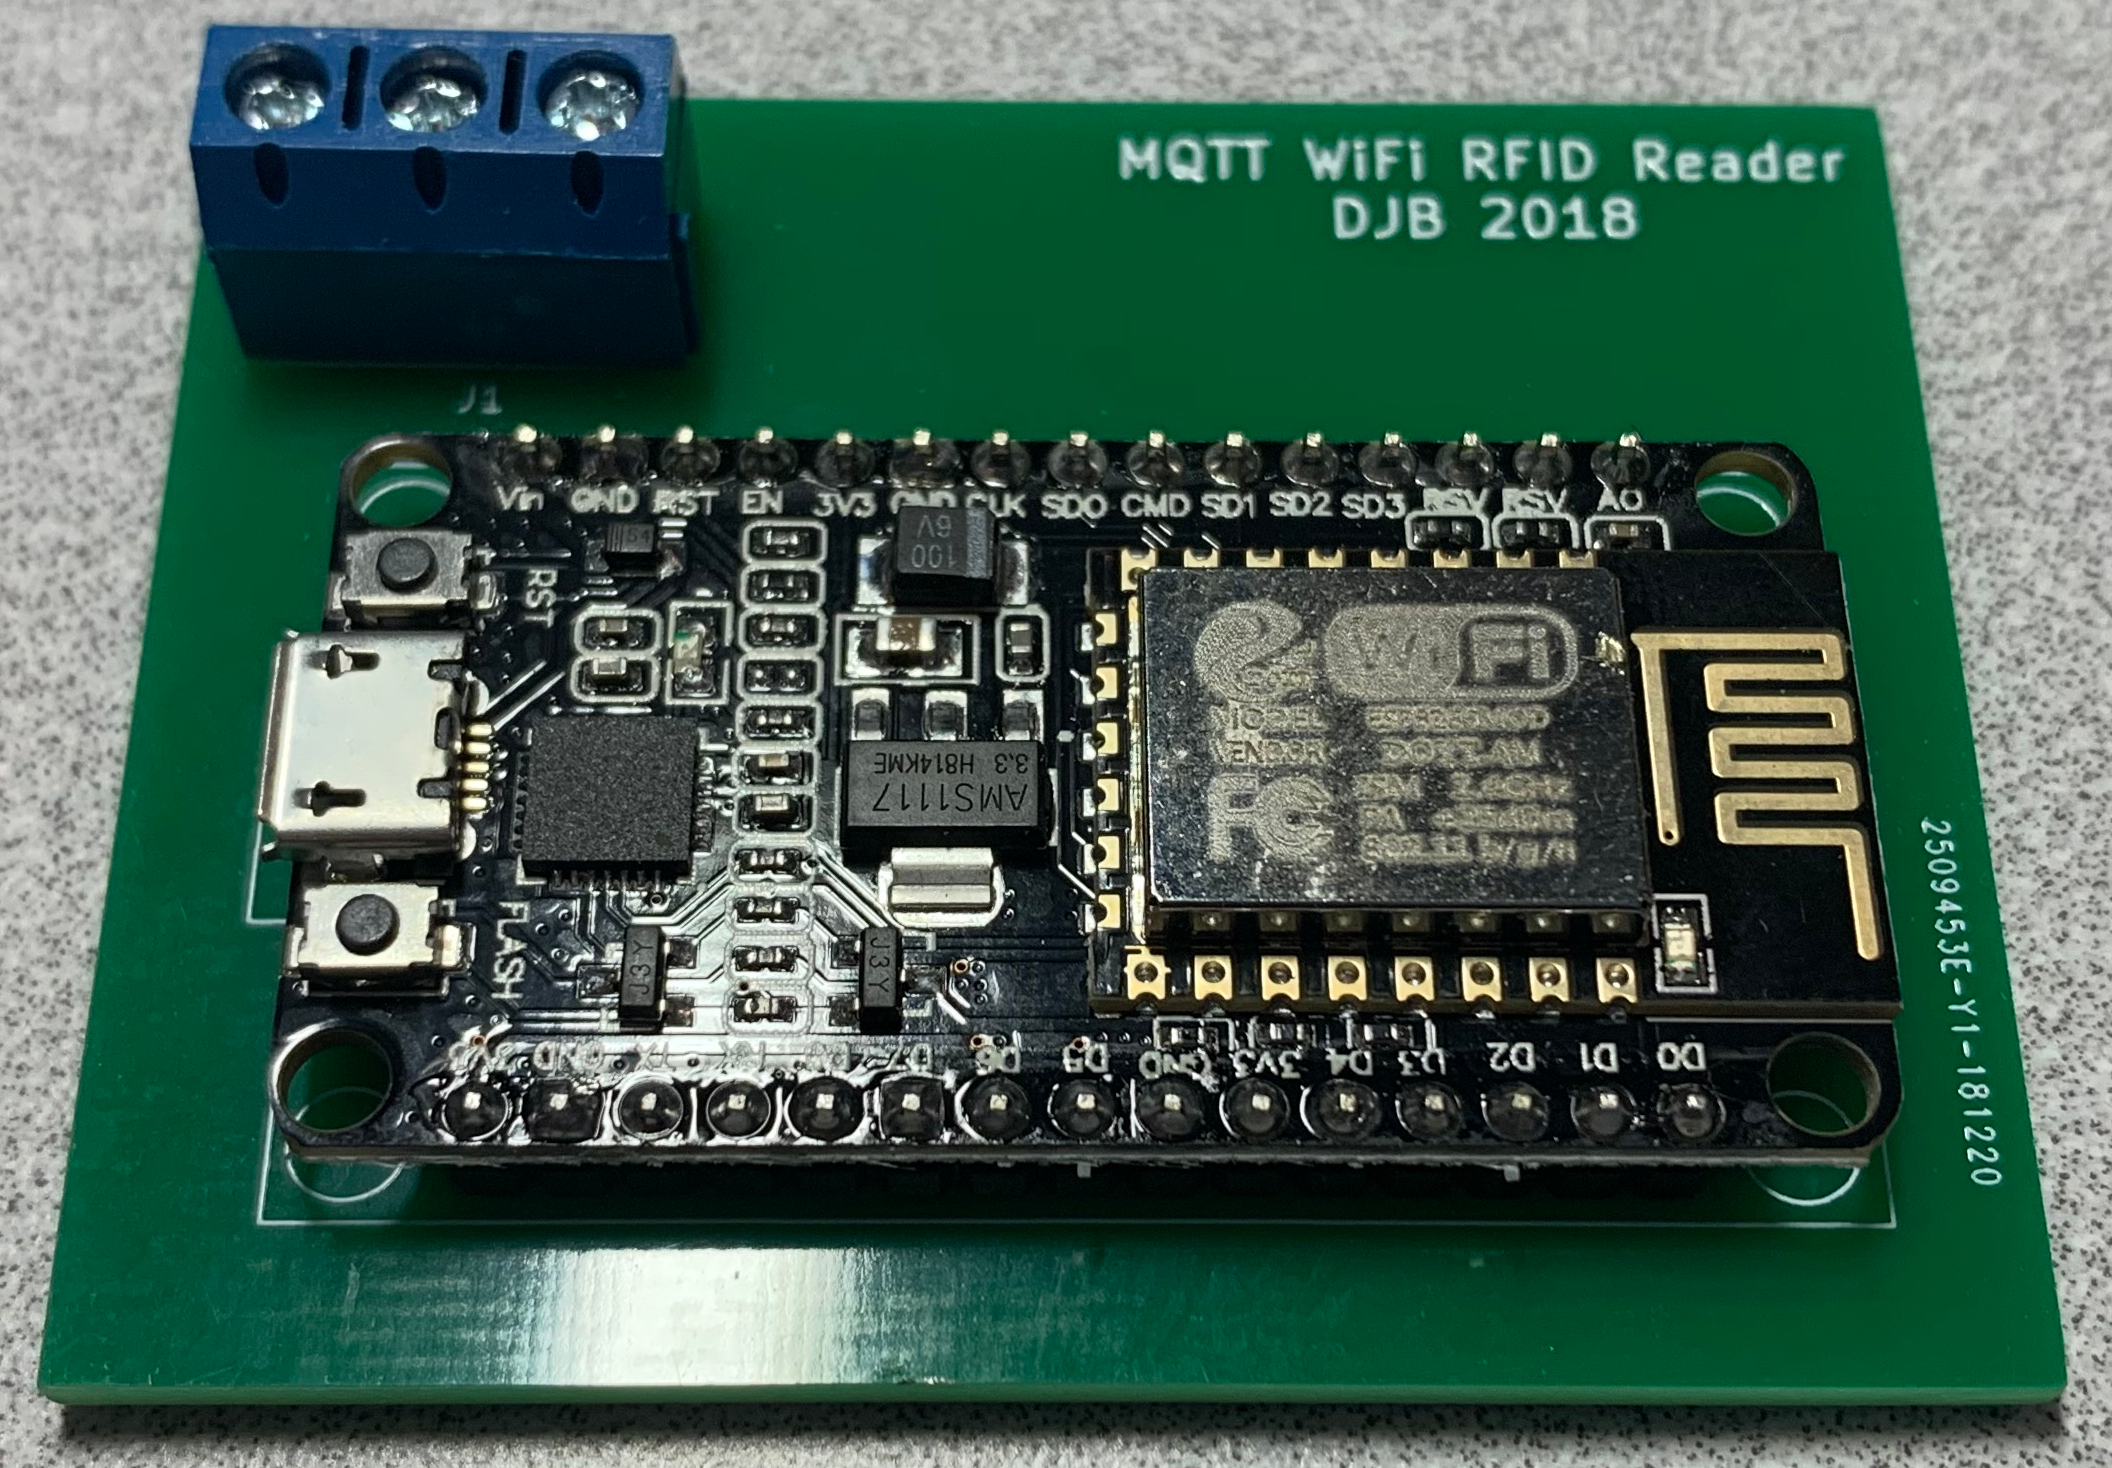
\includegraphics[scale=0.15]{../Images/rfid_pcb.png}
  \caption{RFID Microcontroller PCB}
  \label{fig:rfid_pcb}
\end{figure}
\subsection{Connectivity}
The wiring diagram in Figure \ref{fig:rfid-board} illustrates the connections between the \gls{rfid} readers and the microcontroller. The \gls{rfid} readers are connected to the TB1 terminal block, which uses a RS232 connection to the NodeMCU.
The connections are made using standard wiring techniques, ensuring reliable and secure connections. The use of terminal blocks allows for easy connection and disconnection of the Tortoise machines, making maintenance and troubleshooting easier.
\begin{figure}[H]
  \centering
    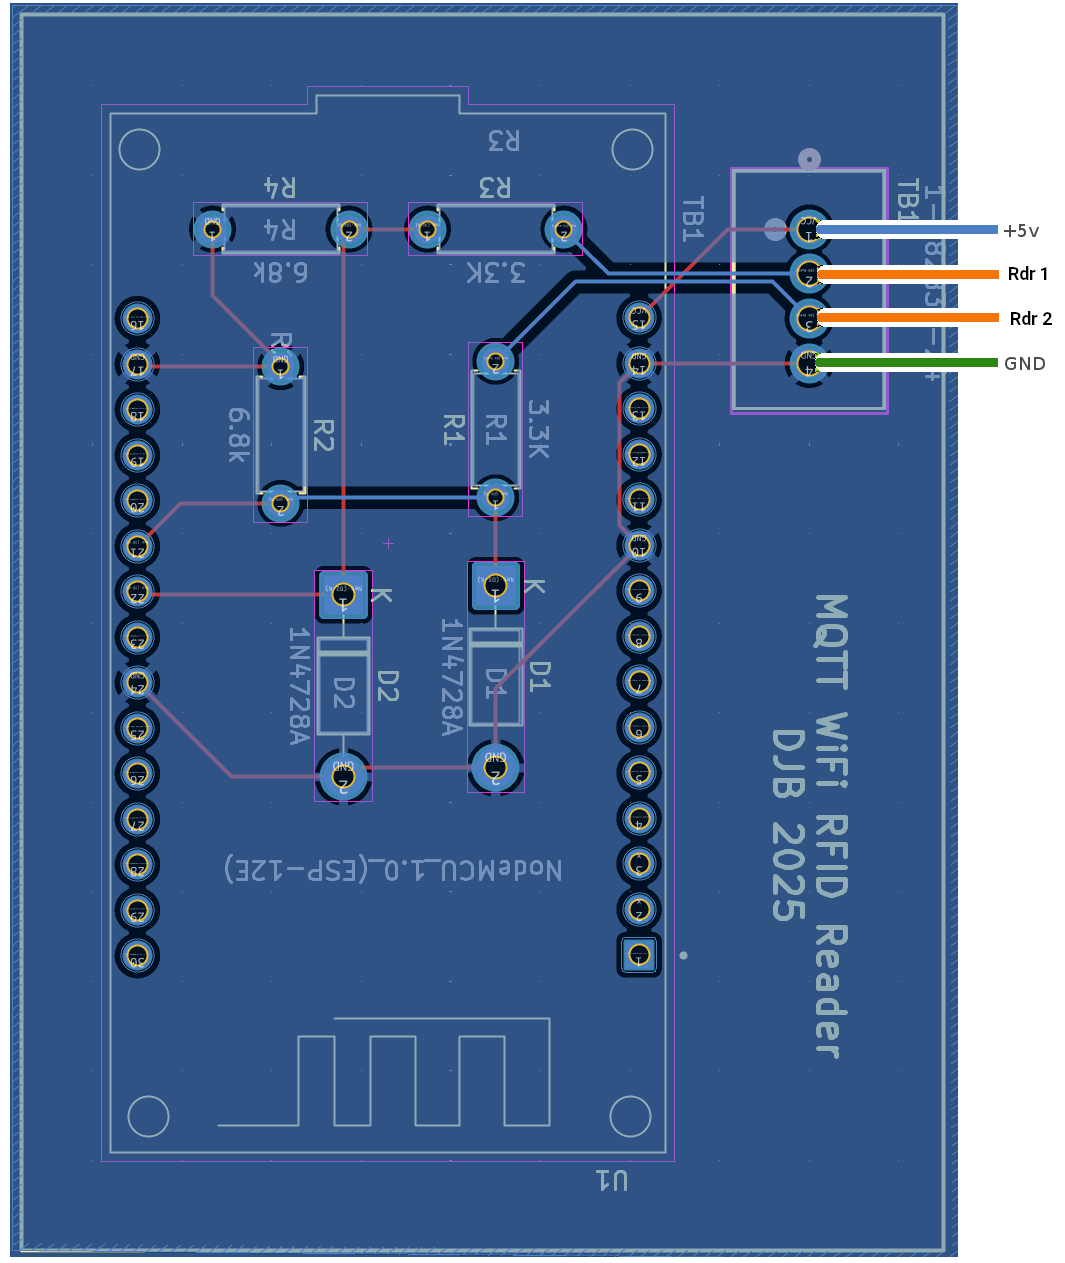
\includegraphics[scale=0.2]{../Images/rfid-board.png}\hfill
    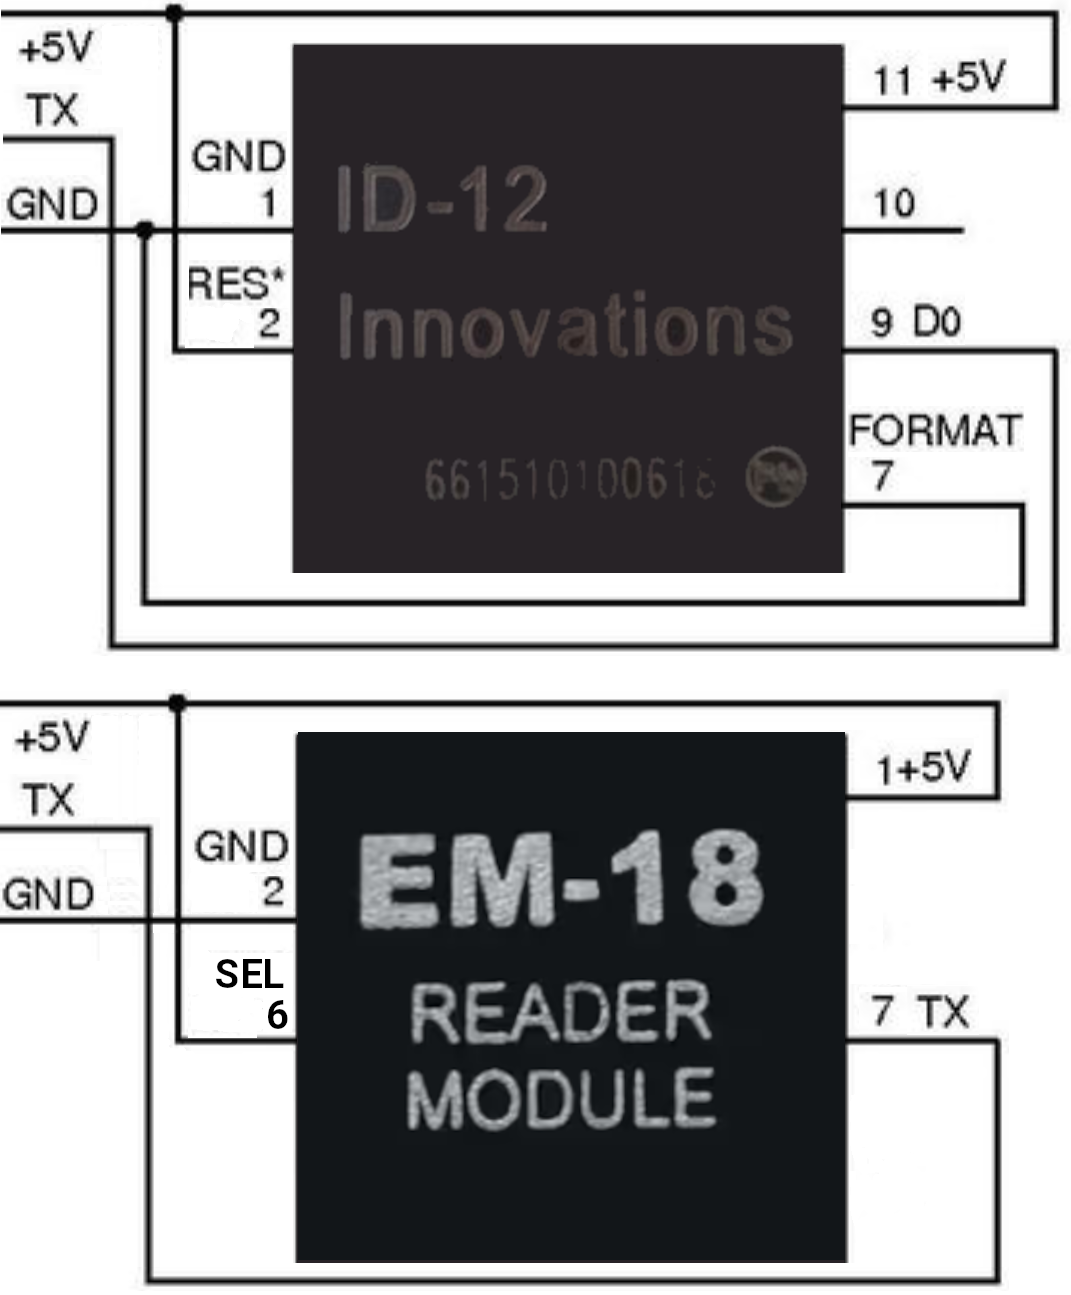
\includegraphics[scale=0.2]{../Images/rfid-readers.png}
  \caption{RFID Microcontroller - RFID Reader Connections}
  \label{fig:rfid-board}
\end{figure}

\section{Software}
The software for the \gls{rfid} microcontroller is developed using the \gls{vscode}, which provides a user-friendly environment for programming microcontrollers. The code is written in C/C++ and utilizes various libraries to facilitate communication with the components.
The software implementation includes the following key functionalities:
\begin{itemize}
  \item Initialization of the NodeMCU and configuration of the GPIO pins.
  \item Initialization of the \gls{wifi} connectivity and connect to the \gls{mqtt} broker. This allows the microcontroller to send and receive messages over the network.
  At the finish of the initialization process, the microcontroller, it will publish a message to the topic ``micros'' indicating its readiness and status to the \gls{mqtt} broker. The message is in \gls{json} format as follows:\\
  \{``et'':``1590462747'',``mcntrlr'':``RfidRdr01'',``msgType'':``initial'',``ip'':``192.168.0.19''\}
\item Setup of the serial communication protocol to interface with the \gls{rfid} reader module. This allows for reading \gls{rfid} tags.
\item Handling \gls{rfid} tag detection and processing the data received from the \gls{rfid} reader. reads values from a single \gls{rfid} reader, formats the results as a \gls{json} string, gets Epoch time from an NTP server and then publishes the \gls{json} String to the topic ``sensors/rfid'' on the \gls{mqtt} broker. The message is in \gls{json} format as follows:\\
\{``et'':``1590463450'',``mcntrlr'':``RfidRdr01'',``reader'':``1'',``rfid'':``1C0044CF23''\}
\item Sending periodic heartbeat messages to the \gls{mqtt} broker to indicate that the microcontroller is operational. This can be used for monitoring and debugging purposes. The message are in \gls{json} format as follows:\\
\{``et'':``1590462747'',``mcntrlr'':``RfidRdr01'',``msgType'':``heartbeat''\}
\end{itemize}
The software is designed to be modular and easily maintainable, allowing for future enhancements and bug fixes. The use of libraries such as ``PubSubClient.h'' for \gls{mqtt} messaging simplifies the implementation and ensures compatibility with the hardware components.

\chapter{Turnout Microcontroller}
\section{Introduction}
A turnout microcontroller is a specialized electronic device designed to control railway turnouts, also known as switches. These devices are essential in model railroading and railway automation, where precise and reliable control
of turnouts is required. By using a microcontroller, it is possible to automate the operation of turnouts, integrate them into larger control systems, and provide feedback on their status. This chapter discusses the design and
implementation of a microcontroller-based system for controlling Tortoise switch machines, which are commonly used in model railroads.
\section{Hardware}
\subsection{Schematic}
The schematic diagram in Figure \ref{fig:turnout-schematic} illustrates the design of the turnout microcontroller circuit. It shows the connections between componentse and the terminal blocks for the Tortoise switch machines. 
Each component is carefully integrated to ensure reliable operation and efficient control of the turnouts. The design also includes capacitors for power supply stabilization and feedback connections for monitoring the switch positions.

\begin{figure}[H]
  \centering
    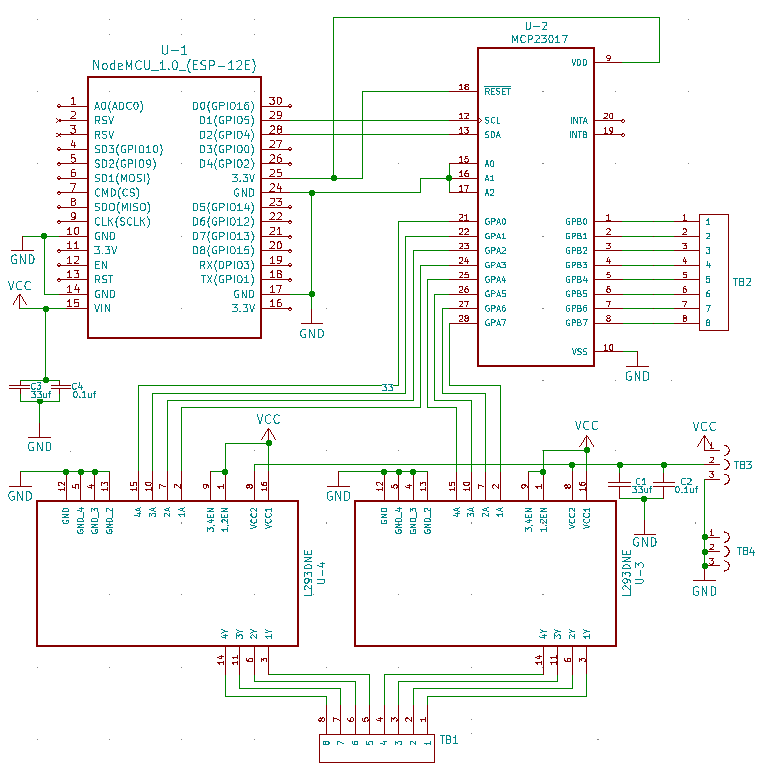
\includegraphics[scale=0.45]{turnout_schematic.png}
  \caption{Turnout Microcontroller Schematic}
  \label{fig:turnout-schematic}
\end{figure}

The hardware used in the turnout microcontroller circuit consists of several components that work together to control the Tortoise switch machines. The main components are:
\begin{itemize}
\item NodeMCU\_1.0\_(ESP-12E) (U-1) is an ESP8266-based development board, which is the controls the other components.
\item MCP23017 (U-2) is a 16-bit I/O expander. It increases the number of GPIO (General Purpose Input/Output) pins available from the NodeMCU. 
\item L293DNE (U-3 and U-4) are dual H-bridge motor drivers. They are used to control the direction of current flow to the Tortoise machines. Tortoise machines require a change in polarity to change the direction of the switch. 
\item TB1 is a terminal block connector where the Tortoise switch machines, up to four, are connected to the circuit. 
\item TB2 is a terminal block connector where the Tortoise switch machines internal contacts are connected to the circuit.
\item TB3 and TB4 are additional terminal blocks, for power distribution. 
\item Capacitors (C1, C2, C3, and C4) are used for filtering and smoothing power supply, ensuring stable operation.
\end{itemize}

The NodeMCU\_1.0\_(ESP-12E) is programmed to control the MCP23017, which in turn controls the L293DNE drivers. The drivers are responsible for controlling the direction of current flow to the Tortoise machines. 
The capacitors are used to filter and smooth the power supply to ensure stable operation of the circuit. The internal contacts of the Tortoise machines are connected to provide feedback on the switch position.
\subsection{PCB Design}
The \gls{pcb} design for the turnout microcontroller is shown in Figure \ref{fig:turnout-board}. The PCB layout is designed to accommodate all the components mentioned in the schematic, ensuring proper 
connections and efficient routing of signals.

\begin{figure}[H]
  \centering
    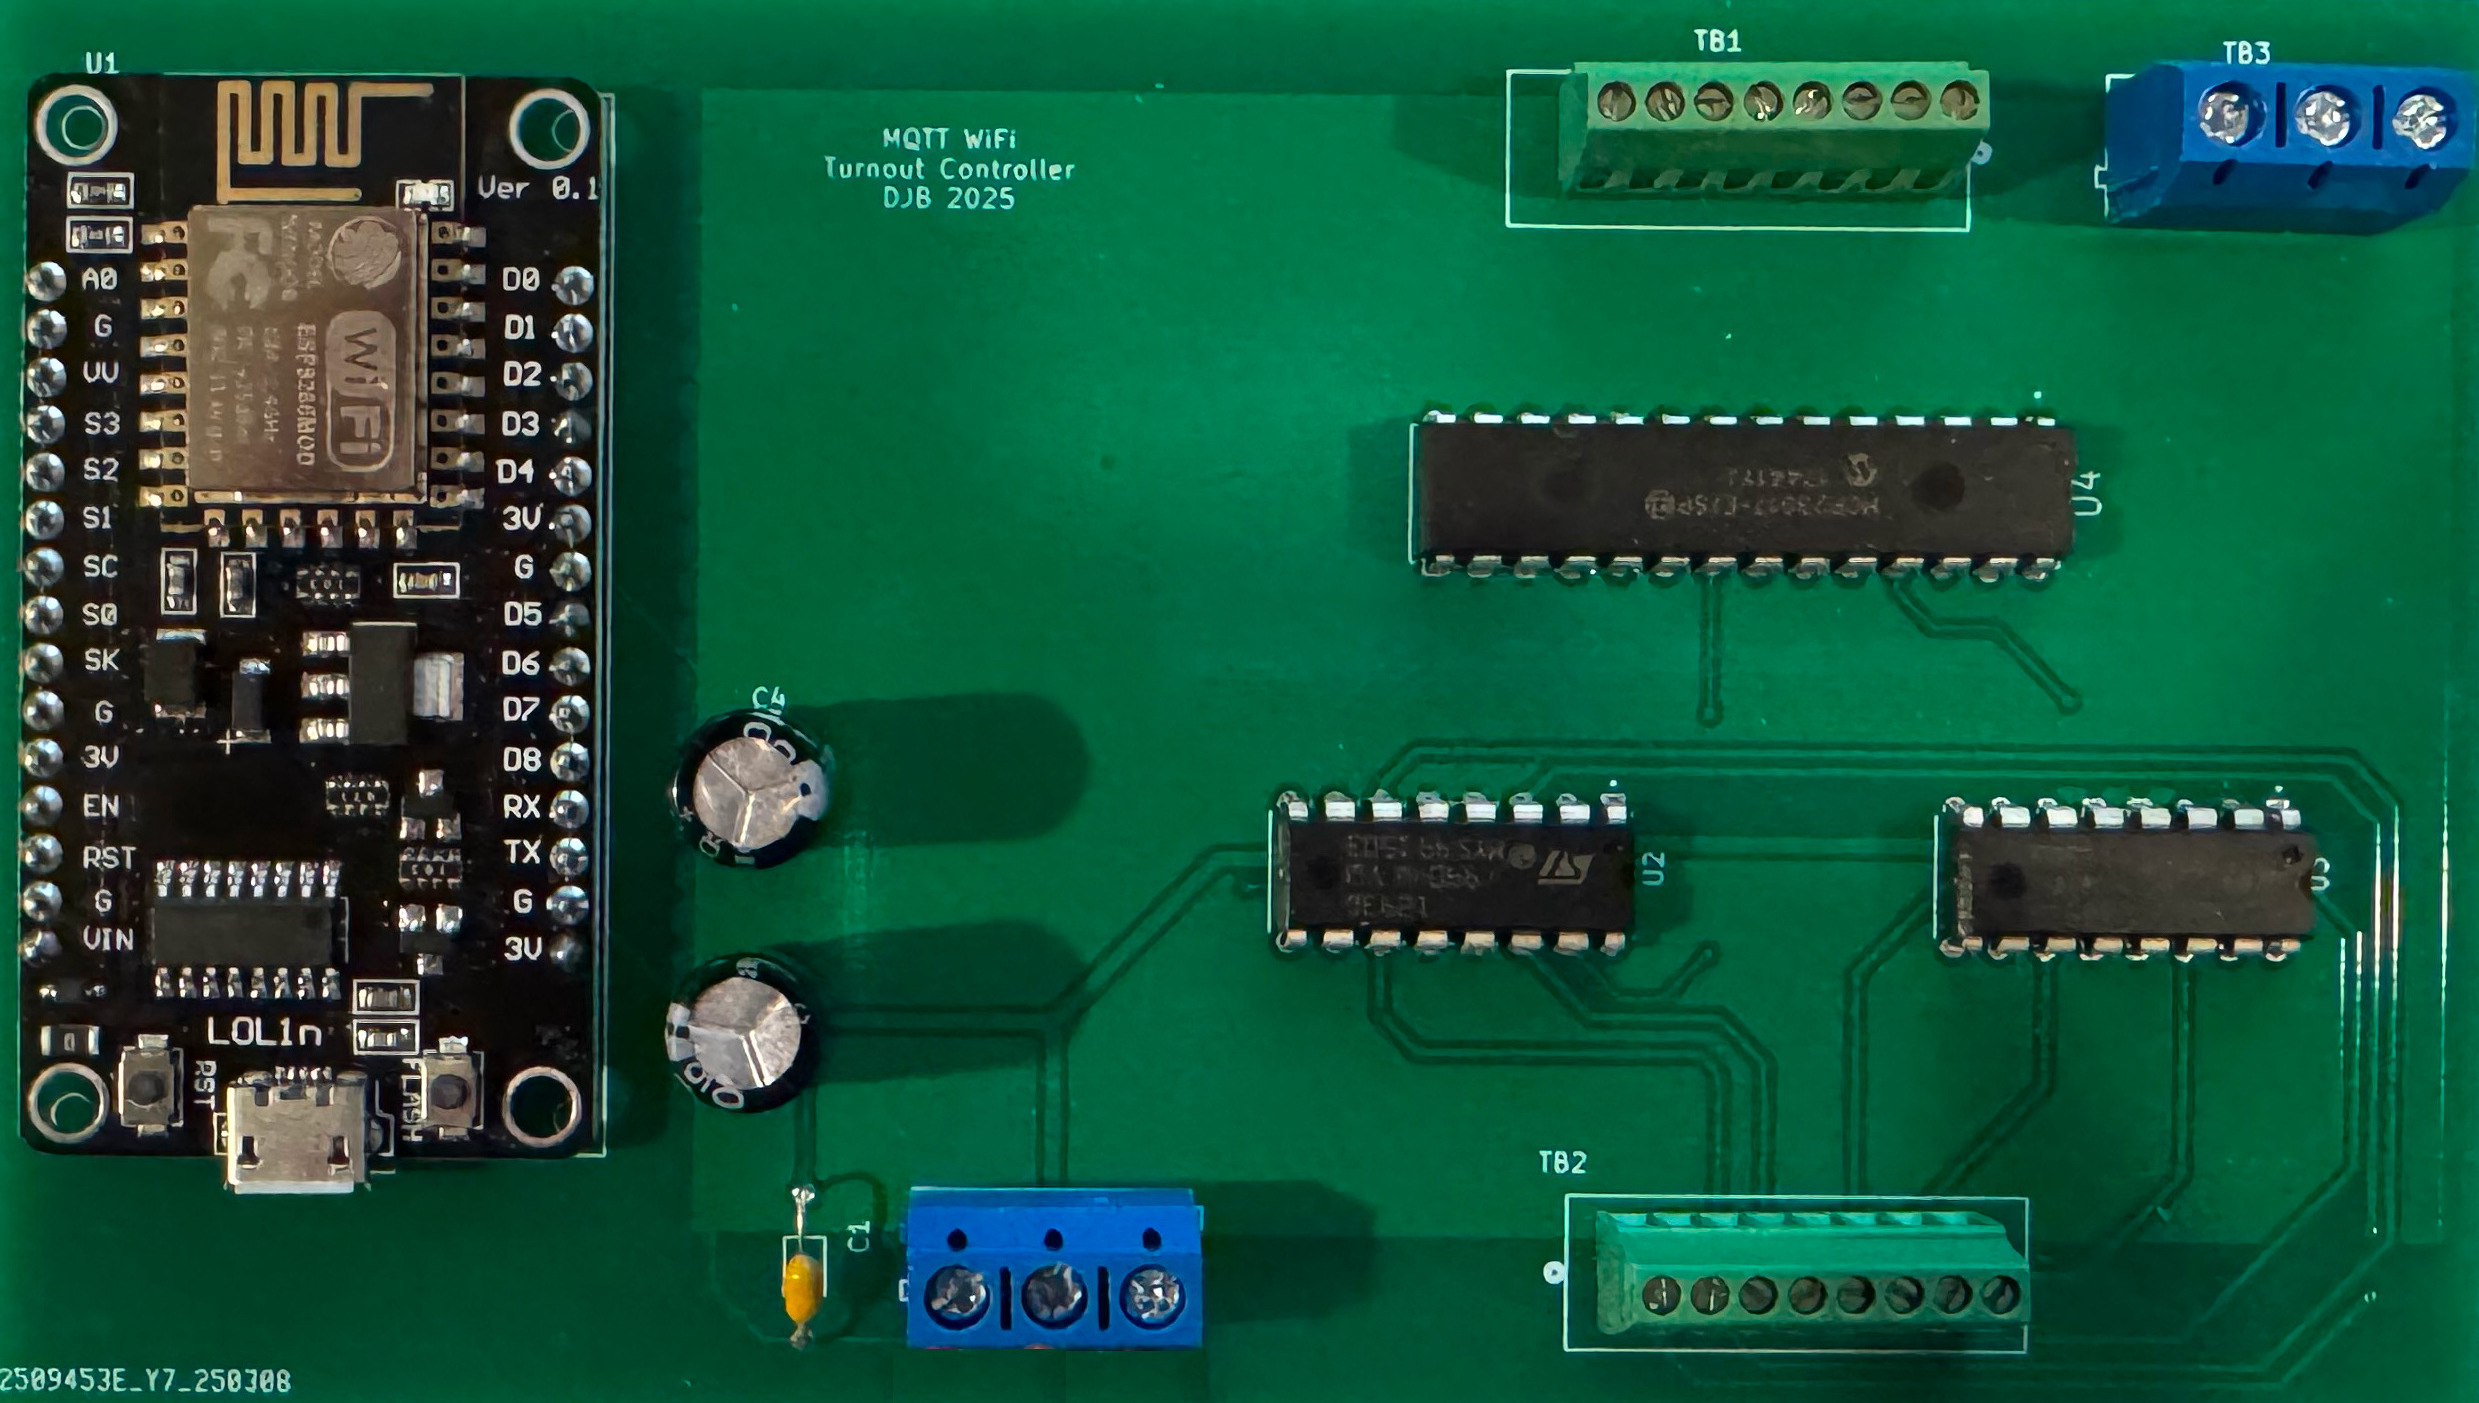
\includegraphics[scale=0.45]{turnout-board.jpg}
  \caption{Turnout Microcontroller PCB}
  \label{fig:turnout-board}
\end{figure}

\subsection{Connectivity}
The wiring diagram in Figure \ref{fig:turnout-board} illustrates the connections between the Tortoise switch machines and the microcontroller. The Tortoise machines are connected to the TB1 terminal block, which is wired to the L293DNE motor drivers.
The internal contacts of the Tortoise machines are connected to the TB2 terminal block, which is wired to the MCP23017 I/O expander. This allows the microcontroller to monitor the position of the switch machines and control their operation.
The connections are made using standard wiring techniques, ensuring reliable and secure connections. The use of terminal blocks allows for easy connection and disconnection of the Tortoise machines, making maintenance and troubleshooting easier.
\begin{figure}[H]
  \centering
    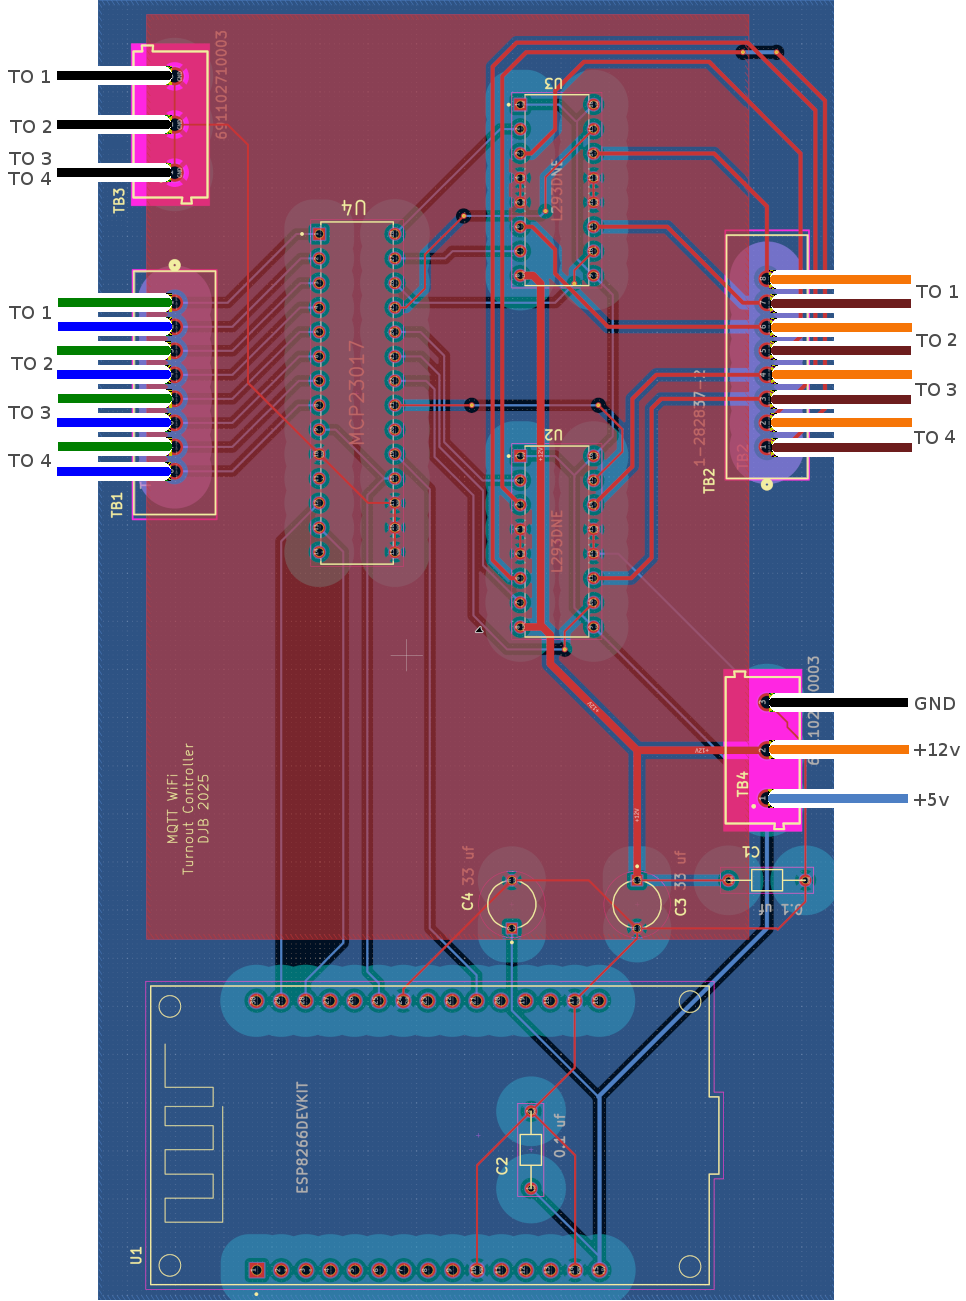
\includegraphics[scale=0.2]{board2.png}\hfill
    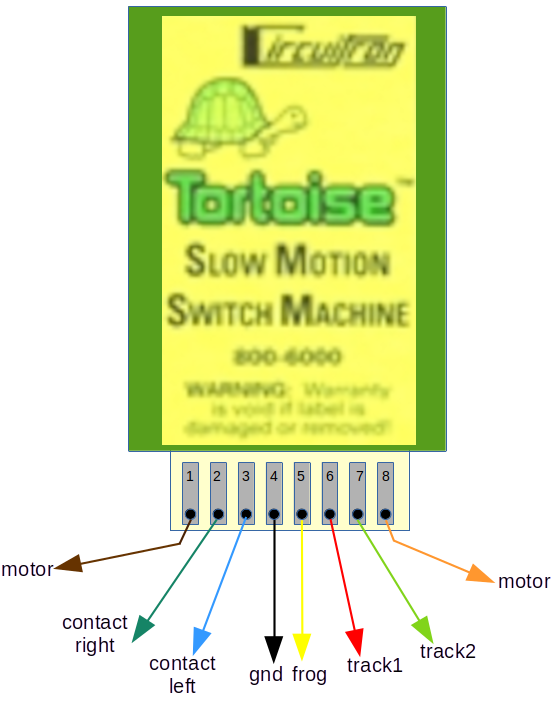
\includegraphics[scale=0.45]{tortoise-wiring.png}
  \caption{Turnout Microcontroller - Tortoise Connections}
  \label{fig:turnout-board}
\end{figure}

\section{Software}
The software for the turnout microcontroller is developed using the \gls{vscode}, which provides a user-friendly environment for programming microcontrollers. The code is written in C/C++ and utilizes various 
libraries to facilitate communication with the components.
The software implementation includes the following key functionalities:
\begin{itemize}
\item Initialization of the NodeMCU and configuration of the GPIO pins.
\item Setup of the \gls{i2c} communication protocol to interface with the MCP23017 I/O expander. This allows for the expansion of GPIO pins beyond what is available on the NodeMCU.
\item Initialization of the \gls{wifi} connectivity and connect to the \gls{mqtt} broker. This allows the microcontroller to send and receive messages over the network.
At the finish of the initialization process, the microcontroller, it will publish a message to the topic "micros" indicating its readiness and status to the \gls{mqtt} broker. The message is in JSON format as follows:\\
\{"et":"1590462747","mcntrlr":"TrnCntlr01","msgType":"initial","ip":"192.168.0.19"\}
\item Subscribes to incoming \gls{mqtt} messages to the topic acts/to/TrnCtlrxx where xx is the this controller's number. This includes parsing commands to throw or close the turnouts or the status of the turnout. 
The commands are in JSON format as follows:\\
\{"cntrlr":"TrnCntlr01","to":"1|2|3|4","cmd":"throw|close|status"\}
\item Communication with the MCP23017 to read the status of the inputs and control the outputs.
\item Implementation of the logic to control the L293DNE motor drivers based on the commands received. This includes setting the appropriate GPIO pins to control the direction and state of the Tortoise machines.
\item Control of the L293DNE motor drivers to change the polarity of the current flow to the Tortoise machines, thereby controlling their position.
\item Monitoring the internal contacts of the Tortoise machines to provide feedback on their position.
\item Handling of any errors or exceptions that may occur during operation, ensuring the system remains stable and responsive.
\item Publishing the status of the turnout positions to an \gls{mqtt} topic for integration with other systems, such as a model railroad control system.The message are in JSON format as follows:\\
\{"et":"1588827073","cntrlr":"trnCtlr01","to":"1","state":"THROWN|CLOSED|ERR|INVLD"\}
where `state` can be `THROWN`, `CLOSED`, `ERR` (for error), or `INVLD` (for invalid state). This allows other components of the system to monitor the status of each turnout in real-time.
\item Sending periodic heartbeat messages to the \gls{mqtt} broker to indicate that the microcontroller is operational. This can be used for monitoring and debugging purposes. The message are in JSON format as follows:\\
\{"et":"1590462747","mcntrlr":"TrnCntlr01","msgType":"heartbeat"\}
\end{itemize}
The software is designed to be modular and easily maintainable, allowing for future enhancements and bug fixes. The use of libraries such as `Wire.h` for I2C communication and `PubSubClient.h` for MQTT messaging simplifies the implementation and ensures compatibility with the hardware components.

%%========================================================================
\backmatter

\printnoidxglossary[sort=letter]
\addcontentsline{toc}{chapter}{Glossary}
\end{document}
